\documentclass[letter,14pt]{article}
\usepackage[utf8]{inputenc}
\usepackage[margin=1in]{geometry}
\usepackage{caption}
\usepackage{multirow,array,varwidth}
\usepackage{lscape}
\usepackage{hyperref}
\usepackage{graphicx}
\usepackage{booktabs}
\usepackage{adjustbox}
\usepackage{float}
\usepackage{appendix}

%opening
\title{The BAW Instruction Set Manual}
\author{Bryant Herren, Austin Waddell, Wesley Ring}
\date{\today}

\newcolumntype{R}[2]{%
    >{\adjustbox{angle=#1,lap=\width-(#2)}\bgroup}%
    l%
    <{\egroup}%
}
\newcommand*\rot{\multicolumn{1}{R{90}{1em}}}% no optional argument here, please!

\begin{document}

\newcommand\DescEntry[1]{%
  \multirow{1}*{%
    \begin{varwidth}{13em}% --- or minipage, if you prefer a fixed width
    \flushright #1%
    \end{varwidth}}}

\newcommand\Tstrut{\rule{0pt}{2.6ex}}       % "top" strut
\newcommand\Bstrut{\rule[-0.9ex]{0pt}{0pt}} % "bottom" strut
\newcommand{\TBstrut}{\Tstrut\Bstrut} % top&bottom struts
    
\null  % Empty line
\nointerlineskip  % No skip for prev line
\vfill
\let\snewpage \newpage
\let\newpage \relax
\maketitle
\let \newpage \snewpage
\vfill 
\newpage

{\hypersetup{linktoc=all,hidelinks}
\tableofcontents
}
\newpage

\section{Introduction}
BAW is the instruction set for a floating point co-processor designed in ECGR 3183 at the University of North Carolina at Charlotte. The co-processor was implemented with a single-cycle architecture, and a pipelined architecture. For the pipelined architecture, two branch prediction algorithms were implemented (1 static and 1 dynamic) as well as no branch prediction.
\newline\newline
Provided in this document:
\begin{itemize}
    \setlength{\parskip}{0pt}
    \setlength{\itemsep}{0pt plus 1pt}
    \item The complete ISA
    \item Architecture and controller design (units, diagrams, etc)
    \item VHDL simulation
    \item Performance results and discussion for pipelined vs. unpipelined approaches
\end{itemize}


\subsection{System Parameters}
\begin{itemize}
    \setlength{\parskip}{0pt}
    \setlength{\itemsep}{0pt plus 1pt}
    \item 32 bits per instruction/register
    \item Data is stored using IEEE single-precision floating point numbers.
    \item Register file has 16 registers
    \item Timings:
    \begin{itemize}
        \setlength{\parskip}{0pt}
        \item Clock cycle (pipelined): 100ns
        \item Register Read/Write: 100ns
        \item Memory Read/Write: 300ns
        \item Single ALU Op: 200ns
    \end{itemize}
\end{itemize}

\subsection{Memory}
The system includes a data memory addressed 0-1023 and 16 Floating Point registers (Referenced as X0-X15). Each memory location and register uses a 32-bit value. The simulation can read an input file containing the operational parameters, code, and memory contents (there is an assembler).
\subsection{Additional Features}
\begin{itemize}
    \setlength{\parskip}{0pt}
    \setlength{\itemsep}{0pt plus 1pt}
    \item FP Multiply by -1, 1, or 0 takes 1 cycle
    \item FP Multiply by power of 2 takes 2 cycles
    \item Condition Codes:
    \begin{itemize}
        \setlength{\parskip}{0pt}
        \setlength{\itemsep}{0pt plus 1pt}
        \item Z - Zero
        \item N - Negative
        \item V - Overflow
        \item C - Carry
        \item E - Error (domain errors, etc.)
    \end{itemize}
    \item All condition codes are set as needed on arithmetic operations
    \item The round, ceiling, and floor functions would round up to the nearest integer, expressing the result in floating point format.
\end{itemize}

\section{ISA}
\subsection{Introduction}
The ISA is based off of the ARMv8 / LEGv8 ISA. As a result, there will likely be similarities.

\subsection{Instruction Format}
There are four instruction formats: Register (R), Data (D), Immediate (I), and Branch (B). 
All processor instructions are 32 bits wide. Table \ref{table:format_descriptions} Contains information about the specific instruction formats.
\newline
\newline
Notes:
\begin{enumerate}
    \item The Opcode is 8 bits long, allowing it to be easily read in hex format. This also allows additional instructions to be added in the future.
    \item 
\end{enumerate}

\begin{table}[H]
\centering
\caption{Instruction Format Descriptions}
\label{table:format_descriptions}
\begin{tabular}{| l | p{7cm} | l |}
\hline
Format & Description & Example \\ \hline
R (Register) & An instruction whose inputs and outputs are both registers & Fadd X9, X21, X9 \\ \hline
D (Data) & An instruction used when fetching or placing data in memory & Load X9, {[}X22, \#64{]} \\ \hline
I (Immediate) & An instruction that carries specific additional data & Pow X9, \#15 \\ \hline
CB (Con. Branch) & An instruction that deals with changing the location of the PC directly, but conditionally & If (Ri == 0) PC $\leftarrow$  LABEL (line) \\ \hline
UB (Unc. Branch) & An instruction that deals with changing the location of the PC directly and unconditionally & PC $\leftarrow$  M[Ri] \\ \hline
S (Set) & An instruction that sets a register to a specific floating point value & Ri $\leftarrow$  FPvalue \\ \hline
\end{tabular}
\end{table}

Please see Table \ref{table:instruction_formats} for specific information on the Instruction Formats.

\begin{landscape}
\begin{table}
\setlength\tabcolsep{4pt}
\caption{Instruction Formats}
\label{table:instruction_formats}
\begin{tabular}{|l|l|l|l|l|l|l|l|l|l|l|l|l|l|l|l|l|l|l|l|l|l|l|l|l|l|l|l|l|l|l|l|l|}
\hline
Instruction Format & 31 & 30 & 29 & 28 & 27 & 26 & 25 & 24 & 23 & 22 & 21 & 20 & 19 & 18 & 17 & 16 & 15 & 14 & 13 & 12 & 11 & 10 & 9 & 8 & 7 & 6 & 5 & 4 & 3 & 2 & 1 & 0 \\ \hline
R (Register) & \multicolumn{8}{l|}{Opcode (8 bits)} & \multicolumn{4}{l|}{Rm (4 bits)} & \multicolumn{12}{l|}{Empty (12 bits)} & \multicolumn{4}{l|}{Rn (4 bits)} & \multicolumn{4}{l|}{Rd (4 bits)} \\ \hline
D (Data) & \multicolumn{8}{l|}{Opcode (8 bits)} & \multicolumn{4}{l|}{Rm (4 bits)} & \multicolumn{14}{l|}{Address (14 bits)} & \multicolumn{2}{l|}{op2 (2 bits)} & \multicolumn{4}{l|}{Rd (4 bits)} \\ \hline
I (Immediate) & \multicolumn{8}{l|}{Opcode (8 bits)} & \multicolumn{4}{l|}{Rm (4 bits)} & \multicolumn{16}{l|}{Immediate Data (16 bits)} & \multicolumn{4}{l|}{Rd (4 bits)} \\ \hline
CB (Con. Branch) & \multicolumn{8}{l|}{Opcode (8 bits)} & \multicolumn{4}{l|}{Rm (4 bits)} & \multicolumn{20}{l|}{Address (20 bits)} \\ \hline
UB (Unc. Branch) & \multicolumn{8}{l|}{Opcode (8 bits)} & \multicolumn{4}{l|}{Empty (4 bits)} & \multicolumn{20}{l|}{Address (20 bits)} \\ \hline
\multirow{2}{*}{S (Set)} & \multicolumn{8}{l|}{Opcode (8 bits)} & \multicolumn{20}{l|}{Empty (20 bits)} & \multicolumn{4}{l|}{Rd (4 bits)} \\ \cline{2-33} 
 & \multicolumn{32}{l|}{Floating Point Value (32 bits)} \\ \hline
\end{tabular}
\end{table}
\end{landscape}

\subsection{Instructions}




%=======================================

\subsubsection{Set}
\begin{table}[!h]
\centering
\caption*{Set}
\begin{tabular}{llllll}
ASM & Opcode & Format & Description & Operation & ALU Cycles \\ \hline
\multicolumn{1}{|c|}{Set} & \multicolumn{1}{c|}{00000001} & \multicolumn{1}{c|}{S} & \DescEntry{Sets Ri to given floating point value} \vline & \multicolumn{1}{c|}{Ri $\leftarrow$  FPvalue} & \multicolumn{1}{c|}{1} \TBstrut \\[1em] \hline
\end{tabular}
\end{table}

\begin{itemize}
    \setlength{\parskip}{0pt}
    \setlength{\itemsep}{0pt plus 1pt}
    \setlength{\itemindent}{-4mm}
    \item[] \textbf{ASM Example:} Set Ri, \#FPvalue
\end{itemize}
\begin{itemize}
    \setlength{\parskip}{0pt}
    \setlength{\itemsep}{0pt plus 1pt}
    \setlength{\itemindent}{7mm}
    \item [\textbf{Flags}]
    \item Zero
    \item Negitive
\end{itemize}

\subsubsection{Load}
\begin{table}[!h]
\centering
\caption*{Load}
\begin{tabular}{llllll}
ASM & Opcode & Format & Description & Operation & ALU Cycles \\ \hline
\multicolumn{1}{|c|}{Load} & \multicolumn{1}{c|}{00000010} & \multicolumn{1}{c|}{D} & \DescEntry{Copies Rj from memory and into Ri} \vline & \multicolumn{1}{c|}{Ri $\leftarrow$  M[Rj]} & \multicolumn{1}{c|}{1} \TBstrut \\[1em] \hline
\end{tabular}
\end{table}

\begin{itemize}
    \setlength{\parskip}{0pt}
    \setlength{\itemsep}{0pt plus 1pt}
    \setlength{\itemindent}{-4mm}
    \item[] \textbf{ASM Example:} Load Ri, Rj
\end{itemize}
\begin{itemize}
    \setlength{\parskip}{0pt}
    \setlength{\itemsep}{0pt plus 1pt}
    \setlength{\itemindent}{7mm}
    \item [\textbf{Flags}]
    \item Zero
    \item Negitive
\end{itemize}

\subsubsection{Store}
\begin{table}[!h]
\centering
\caption*{Store}
\begin{tabular}{llllll}
ASM & Opcode & Format & Description & Operation & ALU Cycles \\ \hline
\multicolumn{1}{|c|}{Store} & \multicolumn{1}{c|}{00000011} & \multicolumn{1}{c|}{D} & \DescEntry{Copies data from register Rj into memory} \vline & \multicolumn{1}{c|}{M[Ri] $\leftarrow$  Rj} & \multicolumn{1}{c|}{1} \TBstrut \\[1em] \hline
\end{tabular}
\end{table}

\begin{itemize}
    \setlength{\parskip}{0pt}
    \setlength{\itemsep}{0pt plus 1pt}
    \setlength{\itemindent}{-4mm}
    \item[] \textbf{ASM Example:} Store Ri, Rj
\end{itemize}
\begin{itemize}
    \setlength{\parskip}{0pt}
    \setlength{\itemsep}{0pt plus 1pt}
    \setlength{\itemindent}{7mm}
    \item [\textbf{Flags}]
    \item None
\end{itemize}

\newpage

\subsubsection{Move}
\begin{table}[!h]
\centering
\caption*{Move}
\begin{tabular}{llllll}
ASM & Opcode & Format & Description & Operation & ALU Cycles \\ \hline
\multicolumn{1}{|c|}{Move} & \multicolumn{1}{c|}{00000100} & \multicolumn{1}{c|}{R} & \DescEntry{Moves the value of Rj to Ri, deleting the original} \vline & \multicolumn{1}{c|}{Ri $\leftarrow$  Rj} & \multicolumn{1}{c|}{1} \TBstrut \\[1em] \hline
\end{tabular}
\end{table}

\begin{itemize}
    \setlength{\parskip}{0pt}
    \setlength{\itemsep}{0pt plus 1pt}
    \setlength{\itemindent}{-4mm}
    \item[] \textbf{ASM Example:} Move Ri, Rj
\end{itemize}
\begin{itemize}
    \setlength{\parskip}{0pt}
    \setlength{\itemsep}{0pt plus 1pt}
    \setlength{\itemindent}{7mm}
    \item [\textbf{Flags}]
    \item Zero
    \item Negitive
\end{itemize}

\subsubsection{Add}
\begin{table}[!h]
\centering
\caption*{Fadd}
\begin{tabular}{llllll}
ASM & Opcode & Format & Description & Operation & ALU Cycles \\ \hline
\multicolumn{1}{|c|}{Fadd} & \multicolumn{1}{c|}{00000101} & \multicolumn{1}{c|}{R} & \DescEntry{Adds Rj and Rk into Ri} \vline & \multicolumn{1}{c|}{Ri $\leftarrow$  Rj + Rk} & \multicolumn{1}{c|}{3} \TBstrut \\[1em] \hline
\end{tabular}
\end{table}

\begin{itemize}
    \setlength{\parskip}{0pt}
    \setlength{\itemsep}{0pt plus 1pt}
    \setlength{\itemindent}{-4mm}
    \item[] \textbf{ASM Example:} Fadd Ri, Rj, Rk
\end{itemize}
\begin{itemize}
    \setlength{\parskip}{0pt}
    \setlength{\itemsep}{0pt plus 1pt}
    \setlength{\itemindent}{7mm}
    \item [\textbf{Flags}]
    \item Zero
    \item Negitive
    \item Overflow
    \item Carry
\end{itemize}

\subsubsection{Subtract}
\begin{table}[!h]
\centering
\caption*{Fsub}
\begin{tabular}{llllll}
ASM & Opcode & Format & Description & Operation & ALU Cycles \\ \hline
\multicolumn{1}{|c|}{Fsub} & \multicolumn{1}{c|}{00000110} & \multicolumn{1}{c|}{R} & \DescEntry{Subtrcts Rk from Rj into Ri} \vline & \multicolumn{1}{c|}{Ri $\leftarrow$  Rj – Rk} & \multicolumn{1}{c|}{3} \TBstrut \\[1em] \hline
\end{tabular}
\end{table}

\begin{itemize}
    \setlength{\parskip}{0pt}
    \setlength{\itemsep}{0pt plus 1pt}
    \setlength{\itemindent}{-4mm}
    \item[] \textbf{ASM Example:} Fsub Ri, Rj, Rk
\end{itemize}
\begin{itemize}
    \setlength{\parskip}{0pt}
    \setlength{\itemsep}{0pt plus 1pt}
    \setlength{\itemindent}{7mm}
    \item [\textbf{Flags}]
    \item Zero
    \item Negitive
    \item Overflow
    \item Carry
\end{itemize}

\newpage

\subsubsection{Negate}
\begin{table}[!h]
\centering
\caption*{Fneg}
\begin{tabular}{llllll}
ASM & Opcode & Format & Description & Operation & ALU Cycles \\ \hline
\multicolumn{1}{|c|}{Fneg} & \multicolumn{1}{c|}{00000111} & \multicolumn{1}{c|}{R} & \DescEntry{Sets Ri to the Opposite of Rj} \vline & \multicolumn{1}{c|}{Ri $\leftarrow$  -Rj} & \multicolumn{1}{c|}{1} \TBstrut \\[1em] \hline
\end{tabular}
\end{table}

\begin{itemize}
    \setlength{\parskip}{0pt}
    \setlength{\itemsep}{0pt plus 1pt}
    \setlength{\itemindent}{-4mm}
    \item[] \textbf{ASM Example:} Fneg Ri, Rj
\end{itemize}
\begin{itemize}
    \setlength{\parskip}{0pt}
    \setlength{\itemsep}{0pt plus 1pt}
    \setlength{\itemindent}{7mm}
    \item [\textbf{Flags}]
    \item Zero
    \item Negitive
\end{itemize}

\subsubsection{Multiply}
\begin{table}[!h]
\centering
\caption*{Fmul}
\begin{tabular}{llllll}
ASM & Opcode & Format & Description & Operation & ALU Cycles \\ \hline
\multicolumn{1}{|c|}{Fmul} & \multicolumn{1}{c|}{00001000} & \multicolumn{1}{c|}{R} & \DescEntry{Multiplies Rj and Rk into Ri} \vline & \multicolumn{1}{c|}{Ri $\leftarrow$  Rj * Rk} & \multicolumn{1}{c|}{5} \TBstrut \\[1em] \hline
\end{tabular}
\end{table}

\begin{itemize}
    \setlength{\parskip}{0pt}
    \setlength{\itemsep}{0pt plus 1pt}
    \setlength{\itemindent}{-4mm}
    \item[] \textbf{ASM Example:} Fmul Ri, Rj, Rk
\end{itemize}
\begin{itemize}
    \setlength{\parskip}{0pt}
    \setlength{\itemsep}{0pt plus 1pt}
    \setlength{\itemindent}{7mm}
    \item [\textbf{Flags}]
    \item Zero
    \item Negitive
    \item Overflow
    \item Carry
\end{itemize}

\subsubsection{Divide}
\begin{table}[!h]
\centering
\caption*{Fdiv}
\begin{tabular}{llllll}
ASM & Opcode & Format & Description & Operation & ALU Cycles \\ \hline
\multicolumn{1}{|c|}{Fdiv} & \multicolumn{1}{c|}{00001001} & \multicolumn{1}{c|}{R} & \DescEntry{Divides Rj by Rk into Ri} \vline & \multicolumn{1}{c|}{Ri $\leftarrow$  Rj / Rk} & \multicolumn{1}{c|}{8} \TBstrut \\[1em] \hline
\end{tabular}
\end{table}

\begin{itemize}
    \setlength{\parskip}{0pt}
    \setlength{\itemsep}{0pt plus 1pt}
    \setlength{\itemindent}{-4mm}
    \item[] \textbf{ASM Example:} Fdiv Ri, Rj, Rk
\end{itemize}
\begin{itemize}
    \setlength{\parskip}{0pt}
    \setlength{\itemsep}{0pt plus 1pt}
    \setlength{\itemindent}{7mm}
    \item [\textbf{Flags}]
    \item Zero
    \item Negitive
    \item Overflow
    \item Carry
    \item Error - divide by zero
\end{itemize}

\newpage

\subsubsection{Floor}
\begin{table}[!h]
\centering
\caption*{Floor}
\begin{tabular}{llllll}
ASM & Opcode & Format & Description & Operation & ALU Cycles \\ \hline
\multicolumn{1}{|c|}{Floor} & \multicolumn{1}{c|}{00001010} & \multicolumn{1}{c|}{R} & \DescEntry{Sets Ri to the floor of Rj} \vline & \multicolumn{1}{c|}{Ri $\leftarrow$  $\lfloor$ Rj$\rfloor$ } & \multicolumn{1}{c|}{1} \TBstrut \\[1em] \hline
\end{tabular}
\end{table}

\begin{itemize}
    \setlength{\parskip}{0pt}
    \setlength{\itemsep}{0pt plus 1pt}
    \setlength{\itemindent}{-4mm}
    \item[] \textbf{ASM Example:} Floor Ri, Rj
\end{itemize}
\begin{itemize}
    \setlength{\parskip}{0pt}
    \setlength{\itemsep}{0pt plus 1pt}
    \setlength{\itemindent}{7mm}
    \item [\textbf{Flags}]
    \item Zero
    \item Negitive
\end{itemize}

\subsubsection{Ceiling}
\begin{table}[!h]
\centering
\caption*{Ceil}
\begin{tabular}{llllll}
ASM & Opcode & Format & Description & Operation & ALU Cycles \\ \hline
\multicolumn{1}{|c|}{Ceil} & \multicolumn{1}{c|}{00001011} & \multicolumn{1}{c|}{R} & \DescEntry{Sets Ri to the ceil of Rj} \vline & \multicolumn{1}{c|}{Ri $\leftarrow$  $\lceil$ Rj$\rceil$ } & \multicolumn{1}{c|}{1} \TBstrut \\[1em] \hline
\end{tabular}
\end{table}

\begin{itemize}
    \setlength{\parskip}{0pt}
    \setlength{\itemsep}{0pt plus 1pt}
    \setlength{\itemindent}{-4mm}
    \item[] \textbf{ASM Example:} Ceil Ri, Rj
\end{itemize}
\begin{itemize}
    \setlength{\parskip}{0pt}
    \setlength{\itemsep}{0pt plus 1pt}
    \setlength{\itemindent}{7mm}
    \item [\textbf{Flags}]
    \item Zero
    \item Negitive
\end{itemize}

\subsubsection{Round}
\begin{table}[!h]
\centering
\caption*{Round}
\begin{tabular}{llllll}
ASM & Opcode & Format & Description & Operation & ALU Cycles \\ \hline
\multicolumn{1}{|c|}{Round} & \multicolumn{1}{c|}{00001100} & \multicolumn{1}{c|}{R} & \DescEntry{Sets Ri to Rj rounded to the nearest integer} \vline & \multicolumn{1}{c|}{Ri $\leftarrow$  round(Rj)} & \multicolumn{1}{c|}{1} \TBstrut \\[1em] \hline
\end{tabular}
\end{table}

\begin{itemize}
    \setlength{\parskip}{0pt}
    \setlength{\itemsep}{0pt plus 1pt}
    \setlength{\itemindent}{-4mm}
    \item[] \textbf{ASM Example:} Round Ri, Rj
\end{itemize}
\begin{itemize}
    \setlength{\parskip}{0pt}
    \setlength{\itemsep}{0pt plus 1pt}
    \setlength{\itemindent}{7mm}
    \item [\textbf{Flags}]
    \item Zero
    \item Negitive
\end{itemize}

\newpage

\subsubsection{Absolute Value}
\begin{table}[!h]
\centering
\caption*{Fabs}
\begin{tabular}{llllll}
ASM & Opcode & Format & Description & Operation & ALU Cycles \\ \hline
\multicolumn{1}{|c|}{Fabs} & \multicolumn{1}{c|}{00001101} & \multicolumn{1}{c|}{R} & \DescEntry{Sets Ri to the absolute value of Rj} \vline & \multicolumn{1}{c|}{Ri $\leftarrow$  | Rj |} & \multicolumn{1}{c|}{1} \TBstrut \\[1em] \hline
\end{tabular}
\end{table}

\begin{itemize}
    \setlength{\parskip}{0pt}
    \setlength{\itemsep}{0pt plus 1pt}
    \setlength{\itemindent}{-4mm}
    \item[] \textbf{ASM Example:} Fabs Ri, Rj
\end{itemize}
\begin{itemize}
    \setlength{\parskip}{0pt}
    \setlength{\itemsep}{0pt plus 1pt}
    \setlength{\itemindent}{7mm}
    \item [\textbf{Flags}]
    \item Zero
\end{itemize}

\subsubsection{Minimum}
\begin{table}[!h]
\centering
\caption*{Min}
\begin{tabular}{llllll}
ASM & Opcode & Format & Description & Operation & ALU Cycles \\ \hline
\multicolumn{1}{|c|}{Min} & \multicolumn{1}{c|}{00001110} & \multicolumn{1}{c|}{R} & \DescEntry{Sets Ri to the minimum value between Rj and Rk} \vline & \multicolumn{1}{c|}{Ri $\leftarrow$  min( Rj, Rk)} & \multicolumn{1}{c|}{1} \TBstrut \\[1em] \hline
\end{tabular}
\end{table}

\begin{itemize}
    \setlength{\parskip}{0pt}
    \setlength{\itemsep}{0pt plus 1pt}
    \setlength{\itemindent}{-4mm}
    \item[] \textbf{ASM Example:} Min Ri, Rj, Rk
\end{itemize}
\begin{itemize}
    \setlength{\parskip}{0pt}
    \setlength{\itemsep}{0pt plus 1pt}
    \setlength{\itemindent}{7mm}
    \item [\textbf{Flags}]
    \item Zero
    \item Negitive
\end{itemize}

\subsubsection{Maximum}
\begin{table}[!h]
\centering
\caption*{Max}
\begin{tabular}{llllll}
ASM & Opcode & Format & Description & Operation & ALU Cycles \\ \hline
\multicolumn{1}{|c|}{Max} & \multicolumn{1}{c|}{00001111} & \multicolumn{1}{c|}{R} & \DescEntry{Sets Ri to the maximum value between Rj and Rk} \vline & \multicolumn{1}{c|}{Ri $\leftarrow$  max( Rj, Rk)} & \multicolumn{1}{c|}{1} \TBstrut \\[1em] \hline
\end{tabular}
\end{table}

\begin{itemize}
    \setlength{\parskip}{0pt}
    \setlength{\itemsep}{0pt plus 1pt}
    \setlength{\itemindent}{-4mm}
    \item[] \textbf{ASM Example:} Max Ri, Rj, Rk
\end{itemize}
\begin{itemize}
    \setlength{\parskip}{0pt}
    \setlength{\itemsep}{0pt plus 1pt}
    \setlength{\itemindent}{7mm}
    \item [\textbf{Flags}]
    \item Zero
    \item Negitive
\end{itemize}

\newpage

\subsubsection{Power}
\begin{table}[!h]
\centering
\caption*{Pow}
\begin{tabular}{llllll}
ASM & Opcode & Format & Description & Operation & ALU Cycles \\ \hline
\multicolumn{1}{|c|}{Pow} & \multicolumn{1}{c|}{00010000} & \multicolumn{1}{c|}{I} & \DescEntry{Sets Ri to Rj raised to some given integer power} \vline & \multicolumn{1}{c|}{Ri $\leftarrow$  Rj\textasciicircum integer\_value} & \multicolumn{1}{c|}{6} \TBstrut \\[1em] \hline
\end{tabular}
\end{table}

\begin{itemize}
    \setlength{\parskip}{0pt}
    \setlength{\itemsep}{0pt plus 1pt}
    \setlength{\itemindent}{-4mm}
    \item[] \textbf{ASM Example:} Pow Ri, Rj, \#integer\_value
\end{itemize}
\begin{itemize}
    \setlength{\parskip}{0pt}
    \setlength{\itemsep}{0pt plus 1pt}
    \setlength{\itemindent}{7mm}
    \item [\textbf{Flags}]
    \item Zero
    \item Negitive
    \item Overflow
    \item Carry
\end{itemize}

\subsubsection{Exponent}
\begin{table}[!h]
\centering
\caption*{Exp}
\begin{tabular}{llllll}
ASM & Opcode & Format & Description & Operation & ALU Cycles \\ \hline
\multicolumn{1}{|c|}{Exp} & \multicolumn{1}{c|}{00010001} & \multicolumn{1}{c|}{R} & \DescEntry{Sets Ri to Rj exponentiated} \vline & \multicolumn{1}{c|}{Ri $\leftarrow$  e\textasciicircum Rj} & \multicolumn{1}{c|}{8} \TBstrut \\[1em] \hline
\end{tabular}
\end{table}

\begin{itemize}
    \setlength{\parskip}{0pt}
    \setlength{\itemsep}{0pt plus 1pt}
    \setlength{\itemindent}{-4mm}
    \item[] \textbf{ASM Example:} Exp Ri, Rj
\end{itemize}
\begin{itemize}
    \setlength{\parskip}{0pt}
    \setlength{\itemsep}{0pt plus 1pt}
    \setlength{\itemindent}{7mm}
    \item [\textbf{Flags}]
    \item Overflow
    \item Carry
\end{itemize}

\subsubsection{Square Root}
\begin{table}[!h]
\centering
\caption*{Sqrt}
\begin{tabular}{llllll}
ASM & Opcode & Format & Description & Operation & ALU Cycles \\ \hline
\multicolumn{1}{|c|}{Sqrt} & \multicolumn{1}{c|}{00010010} & \multicolumn{1}{c|}{R} & \DescEntry{Sets Ri to the square root of Rj} \vline & \multicolumn{1}{c|}{Ri $\leftarrow$  $\surd$ Rj} & \multicolumn{1}{c|}{8} \TBstrut \\[1em] \hline
\end{tabular}
\end{table}

\begin{itemize}
    \setlength{\parskip}{0pt}
    \setlength{\itemsep}{0pt plus 1pt}
    \setlength{\itemindent}{-4mm}
    \item[] \textbf{ASM Example:} Sqrt Ri, Rj
\end{itemize}
\begin{itemize}
    \setlength{\parskip}{0pt}
    \setlength{\itemsep}{0pt plus 1pt}
    \setlength{\itemindent}{7mm}
    \item [\textbf{Flags}]
    \item Zero
    \item Overflow
    \item Carry
    \item Error - complex domain
\end{itemize}

\newpage

\subsubsection{Branch (Uncond.)}
\begin{table}[!h]
\centering
\caption*{B}
\begin{tabular}{llllll}
ASM & Opcode & Format & Description & Operation & ALU Cycles \\ \hline
\multicolumn{1}{|c|}{B} & \multicolumn{1}{c|}{00010011} & \multicolumn{1}{c|}{UB} & \DescEntry{Loads Ri from memory into PC} \vline & \multicolumn{1}{c|}{PC $\leftarrow$  M[Ri]} & \multicolumn{1}{c|}{1} \TBstrut \\[1em] \hline
\end{tabular}
\end{table}

\begin{itemize}
    \setlength{\parskip}{0pt}
    \setlength{\itemsep}{0pt plus 1pt}
    \setlength{\itemindent}{-4mm}
    \item[] \textbf{ASM Example:} B Ri
\end{itemize}
\begin{itemize}
    \setlength{\parskip}{0pt}
    \setlength{\itemsep}{0pt plus 1pt}
    \setlength{\itemindent}{7mm}
    \item [\textbf{Flags}]
    \item None
\end{itemize}

\subsubsection{Branch Zero}
\begin{table}[!h]
\centering
\caption*{BZ}
\begin{tabular}{llllll}
ASM & Opcode & Format & Description & Operation & ALU Cycles \\ \hline
\multicolumn{1}{|c|}{BZ} & \multicolumn{1}{c|}{00010100} & \multicolumn{1}{c|}{CB} & \DescEntry{Sends the PC to a specific labeled line if Ri is zero} \vline & \multicolumn{1}{c|}{If (Ri == 0) PC $\leftarrow$  LABEL (line)} & \multicolumn{1}{c|}{3} \TBstrut \\[1em] \hline
\end{tabular}
\end{table}

\begin{itemize}
    \setlength{\parskip}{0pt}
    \setlength{\itemsep}{0pt plus 1pt}
    \setlength{\itemindent}{-4mm}
    \item[] \textbf{ASM Example:} BZ Ri, LABEL
\end{itemize}
\begin{itemize}
    \setlength{\parskip}{0pt}
    \setlength{\itemsep}{0pt plus 1pt}
    \setlength{\itemindent}{7mm}
    \item [\textbf{Flags}]
    \item Zero
\end{itemize}

\subsubsection{Branch Negative}
\begin{table}[!h]
\centering
\caption*{BN}
\begin{tabular}{llllll}
ASM & Opcode & Format & Description & Operation & ALU Cycles \\ \hline
\multicolumn{1}{|c|}{BN} & \multicolumn{1}{c|}{00010101} & \multicolumn{1}{c|}{CB} & \DescEntry{Sends the PC to a specific labeled line if Ri is negative} \vline & \multicolumn{1}{c|}{If (Ri < 0) PC $\leftarrow$  LABEL (line)} & \multicolumn{1}{c|}{3} \TBstrut \\[1em] \hline
\end{tabular}
\end{table}

\begin{itemize}
    \setlength{\parskip}{0pt}
    \setlength{\itemsep}{0pt plus 1pt}
    \setlength{\itemindent}{-4mm}
    \item[] \textbf{ASM Example:} BN Ri, LABEL
\end{itemize}
\begin{itemize}
    \setlength{\parskip}{0pt}
    \setlength{\itemsep}{0pt plus 1pt}
    \setlength{\itemindent}{7mm}
    \item [\textbf{Flags}]
    \item Negitive
\end{itemize}

\newpage

\subsubsection{No-op}
\begin{table}[!h]
\centering
\caption*{Nop}
\begin{tabular}{llllll}
ASM & Opcode & Format & Description & Operation & ALU Cycles \\ \hline
\multicolumn{1}{|c|}{Nop} & \multicolumn{1}{c|}{00010110} & \multicolumn{1}{c|}{-} & \DescEntry{No operation} \vline & \multicolumn{1}{c|}{No operation} & \multicolumn{1}{c|}{1} \TBstrut \\[1em] \hline
\end{tabular}
\end{table}

\begin{itemize}
    \setlength{\parskip}{0pt}
    \setlength{\itemsep}{0pt plus 1pt}
    \setlength{\itemindent}{-4mm}
    \item[] \textbf{ASM Example:} Nop
\end{itemize}
\begin{itemize}
    \setlength{\parskip}{0pt}
    \setlength{\itemsep}{0pt plus 1pt}
    \setlength{\itemindent}{7mm}
    \item [\textbf{Flags}]
    \item None
\end{itemize}

\subsubsection{Halt}
\begin{table}[!h]
\centering
\caption*{Halt}
\begin{tabular}{llllll}
ASM & Opcode & Format & Description & Operation & ALU Cycles \\ \hline
\multicolumn{1}{|c|}{Halt} & \multicolumn{1}{c|}{00010111} & \multicolumn{1}{c|}{-} & \DescEntry{Stop program} \vline & \multicolumn{1}{c|}{Stop Program} & \multicolumn{1}{c|}{-} \TBstrut \\[1em] \hline
\end{tabular}
\end{table}

\begin{itemize}
    \setlength{\parskip}{0pt}
    \setlength{\itemsep}{0pt plus 1pt}
    \setlength{\itemindent}{-4mm}
    \item[] \textbf{ASM Example:} Halt
\end{itemize}
\begin{itemize}
    \setlength{\parskip}{0pt}
    \setlength{\itemsep}{0pt plus 1pt}
    \setlength{\itemindent}{7mm}
    \item [\textbf{Flags}]
    \item None
\end{itemize}



%========================================
\newpage
\section{Architecture}

\subsection{ALU}
	
The ALU can perform fourteen unique operations, and also pass through input A. Eleven of these operations are done in the second phase of the ALU, directly after the pre-normalization process (Fadd, for example). The remaining three operations are done in the final stage of the ALU, directly after the post-normalization process (Floor, for example). The figure below shows each phase of the ALU in order from input to result.
	
	\begin{figure}[H]
	\begin{center}
	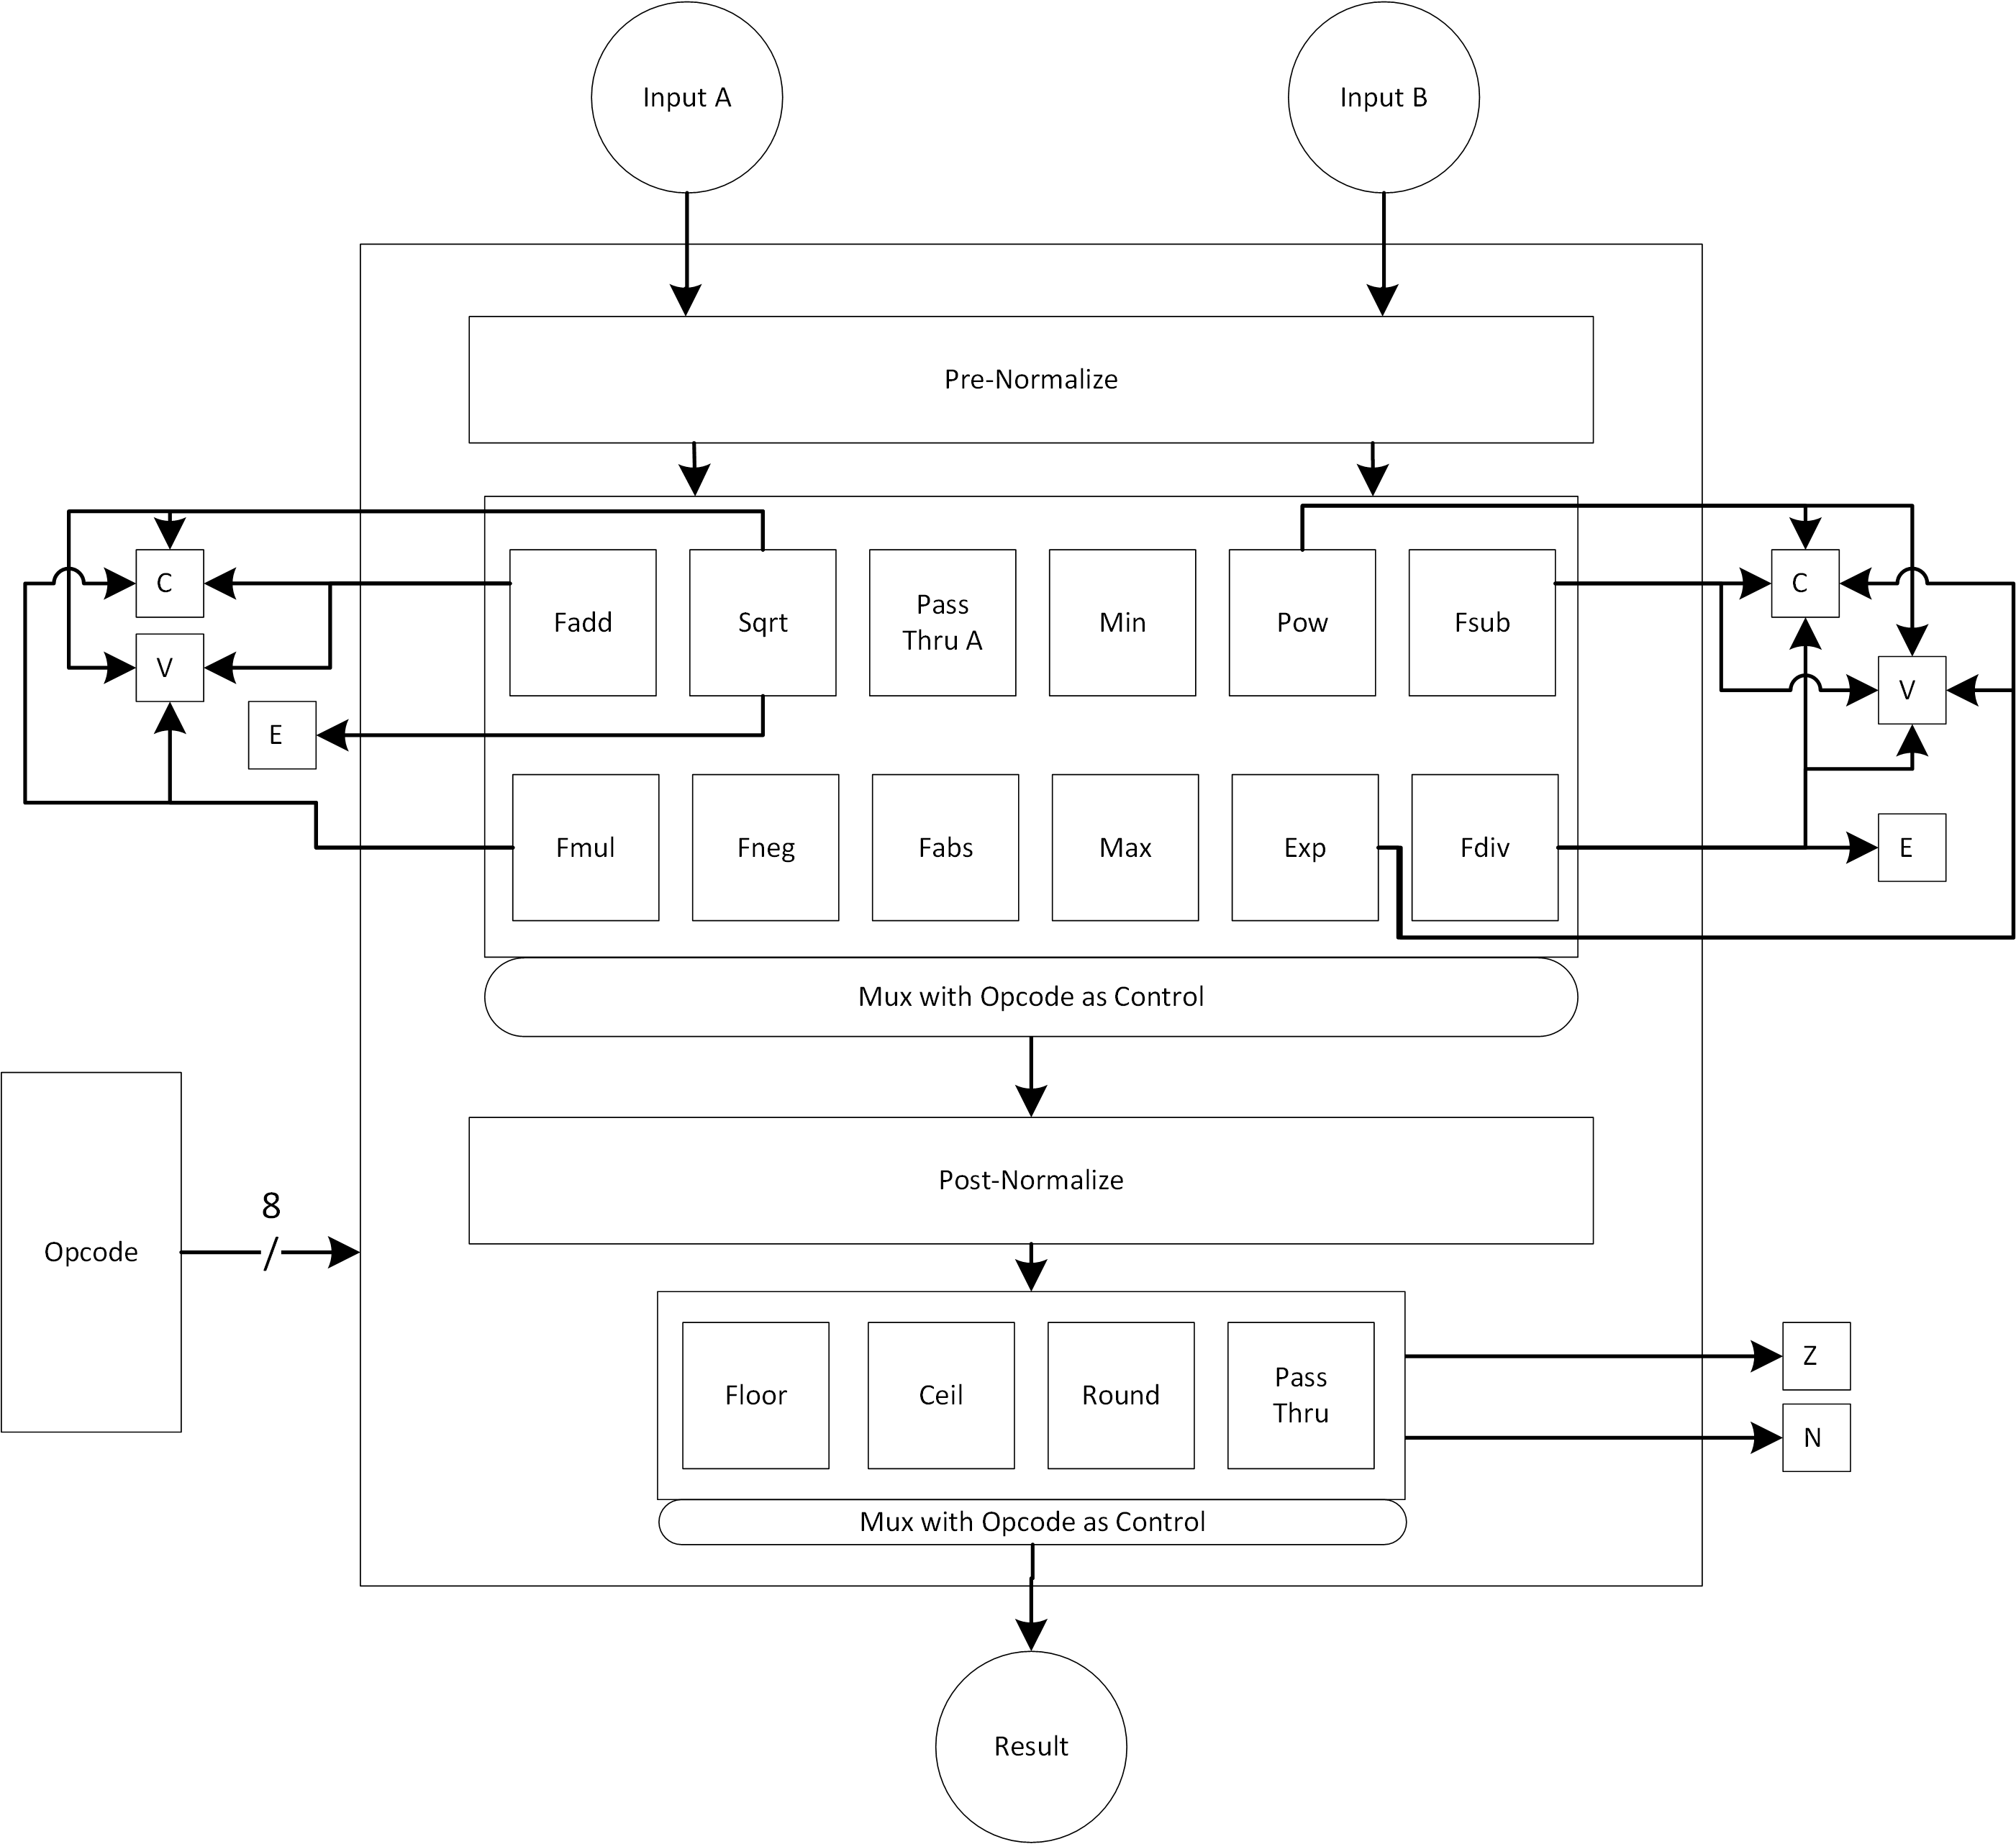
\includegraphics[width=1\linewidth]{ALU.png}
	\caption{ALU Design}
	\end{center}
	\end{figure}
	
\noindent
When the two inputs enter the ALU, their exponents are normalized to whichever input is larger. The larger input is chosen because it’s less likely to result in a loss of precision. Depending on the instruction, the two inputs may bypass the normalization process in order to save on ALU cycles (Fabs, for example).
\noindent\newline\newline
Next is the first stage of arithmetic where the inputs are added, multiplied, etc. The functional blocks of this section can out any combination of the following three flags: carry, overflow, and error. The figure above depicts specifically what blocks can trigger what flags. The error flag is exclusively used for domain errors, either when dividing by zero or entering the complex domain.
 \noindent\newline\newline
After the first stage of arithmetic, the result enters the post-normalize stage (which can be bypassed like before) and then is passed through to the result output of the ALU. This is also where the zero and negative flags are set if necessary. Alternatively, if the first stage of arithmetic is skipped (pass-through), then the second stage may be used for the Round, Floor, and Ceil functions. It's worth noting that having two stages of arithmetic allows for combination instructions to be implemented with little to no additional hardware (Fadd + Round, for example) in order to make the common case fast. This is why more Opcode bits than necessary exist.
 \noindent\newline\newline
The entire ALU is controlled by the Opcode control signal, which comes directly out of the instruction. See Table \ref{table:datapath_control} to determine which Opcodes correspond to which ALU functions.


\subsection{Datapath}
	\subsubsection{Single Cycle}
	Blah Blah Blah Blah Blah Blah Blah Blah Blah Blah Blah Blah Blah Blah Blah Blah Blah Blah Blah Blah Blah Blah Blah Blah Blah 
	\begin{figure}[H]
	\begin{center}
	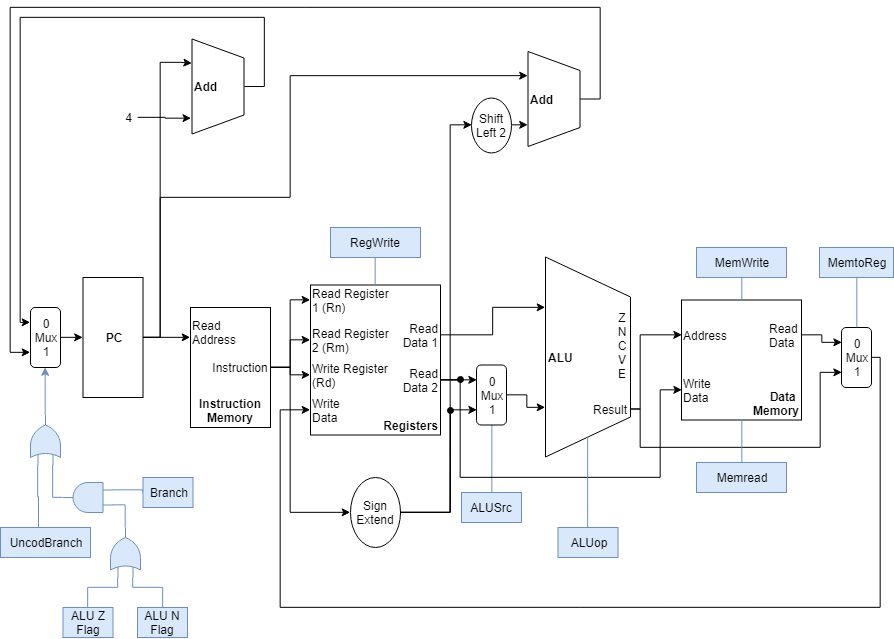
\includegraphics[width=1\linewidth]{SingleCycleArch.png}
	\caption{Single Cycle Architecture}
	\end{center}
	\end{figure}
	\noindent
	Blah Blah Blah Blah Blah Blah Blah Blah Blah Blah Blah Blah Blah Blah Blah Blah Blah Blah Blah Blah Blah Blah Blah Blah Blah 
	
	\newpage
	\subsubsection{Pipelined}
	Blah Blah Blah Blah Blah Blah Blah Blah Blah Blah Blah Blah Blah Blah Blah Blah Blah Blah Blah Blah Blah Blah Blah Blah Blah 
	\begin{figure}[H]
	\begin{center}
	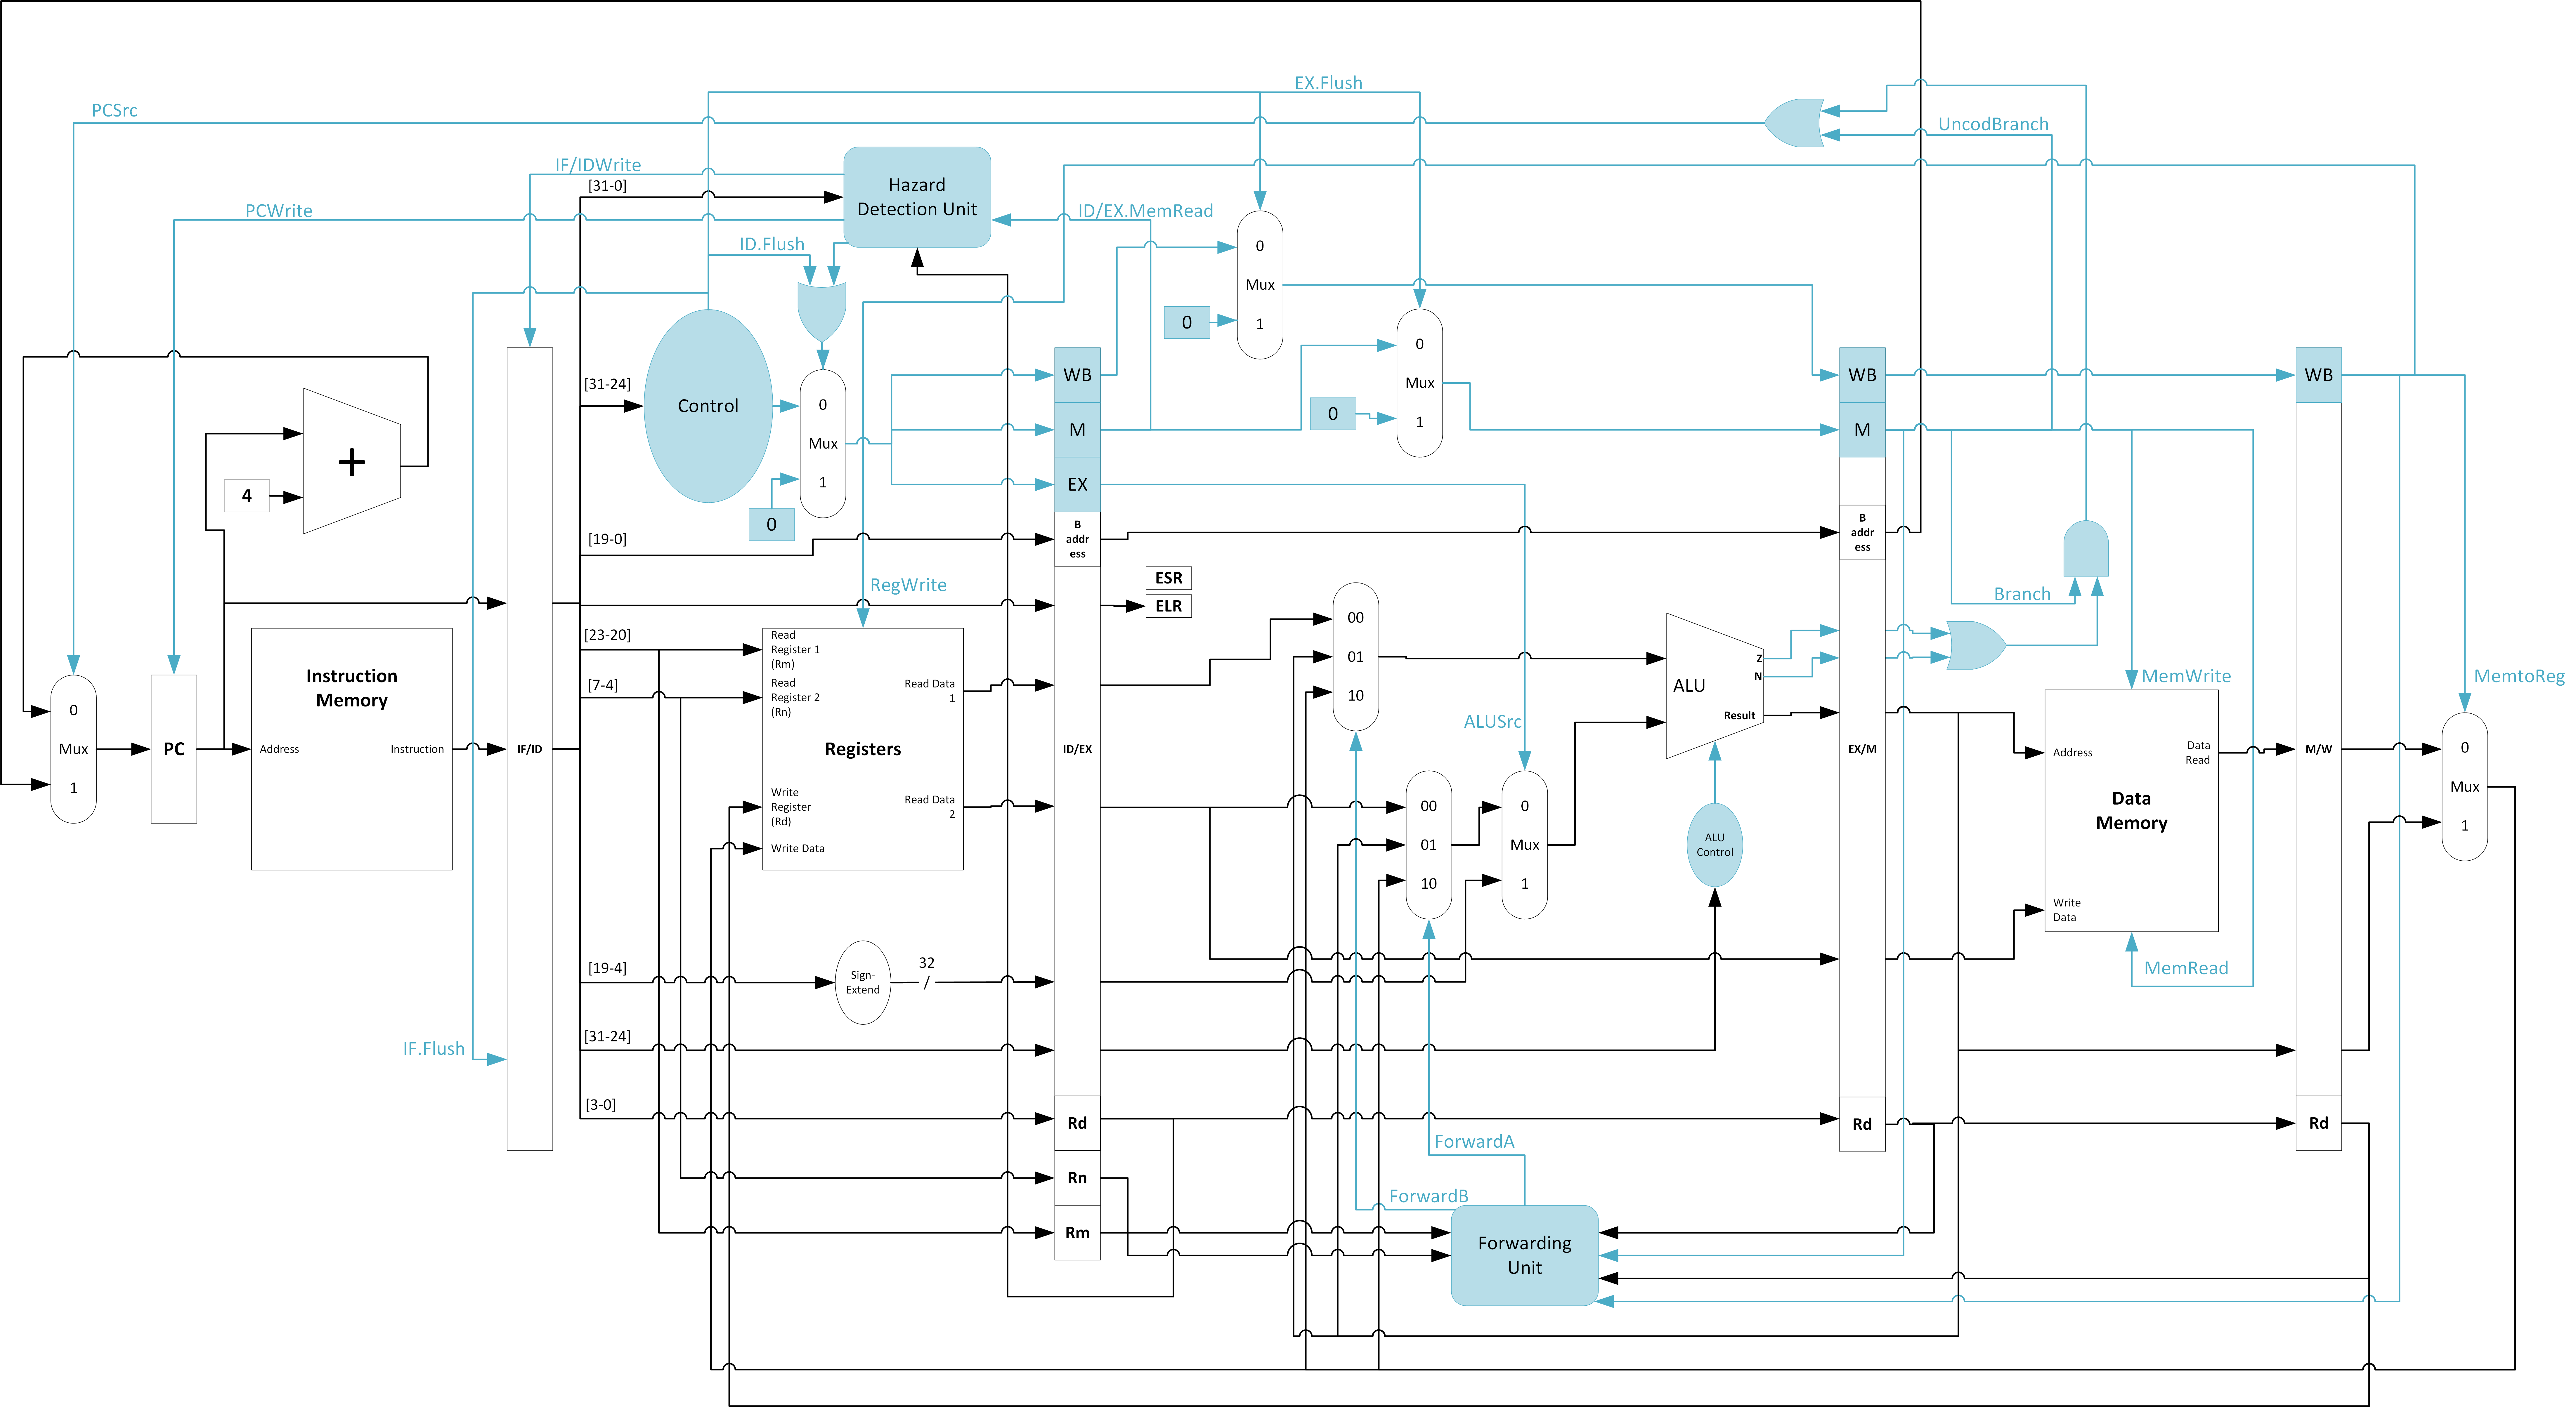
\includegraphics[width=1\linewidth]{PipelinedArch.png}
	\caption{Pipelined Architecture}
	\end{center}
	\end{figure}
	\noindent
	Blah Blah Blah Blah Blah Blah Blah Blah Blah Blah Blah Blah Blah Blah Blah Blah Blah Blah Blah Blah Blah Blah Blah Blah Blah 


\subsection{Controller}
Blah Blah Blah Blah Blah Blah Blah Blah Blah Blah Blah Blah Blah Blah Blah Blah Blah Blah Blah Blah Blah Blah Blah Blah Blah 
\begin{table}[H]
\centering
\caption{Datapath Control}
\label{table:datapath_control}
\begin{tabular}{lllllllllll}
ASM & Opcode & \rot{ALUSrc} & \rot{MemtoReg} & \rot{RegWrite} & \rot{MemRead} & \rot{MemWrite} & \rot{Branch} & \rot{UncodBranch} & ALU Control Description  \\ \hline
\multicolumn{1}{|c|}{Set} & \multicolumn{1}{c|}{00000001} & \multicolumn{1}{c|}{1} & \multicolumn{1}{c|}{0} & \multicolumn{1}{c|}{1} & \multicolumn{1}{c|}{0} & \multicolumn{1}{c|}{0} & \multicolumn{1}{c|}{0} & \multicolumn{1}{c|}{0} & \multicolumn{1}{c|}{Use Adder} \TBstrut \\[1em] \hline
\multicolumn{1}{|c|}{Load} & \multicolumn{1}{c|}{00000010} & \multicolumn{1}{c|}{1} & \multicolumn{1}{c|}{1} & \multicolumn{1}{c|}{1} & \multicolumn{1}{c|}{1} & \multicolumn{1}{c|}{0} & \multicolumn{1}{c|}{0} & \multicolumn{1}{c|}{0} & \multicolumn{1}{c|}{Use Adder} \TBstrut \\[1em] \hline
\multicolumn{1}{|c|}{Store} & \multicolumn{1}{c|}{00000011} & \multicolumn{1}{c|}{1} & \multicolumn{1}{c|}{X} & \multicolumn{1}{c|}{0} & \multicolumn{1}{c|}{0} & \multicolumn{1}{c|}{1} & \multicolumn{1}{c|}{0} & \multicolumn{1}{c|}{0} & \multicolumn{1}{c|}{Use Adder} \TBstrut \\[1em] \hline

\multicolumn{1}{|c|}{Move} & \multicolumn{1}{c|}{00000100} & \multicolumn{1}{c|}{0} & \multicolumn{1}{c|}{0} & \multicolumn{1}{c|}{1} & \multicolumn{1}{c|}{0} & \multicolumn{1}{c|}{0} & \multicolumn{1}{c|}{0} & \multicolumn{1}{c|}{0} & \multicolumn{1}{c|}{Pass Through} \TBstrut \\[1em] \hline 
\multicolumn{1}{|c|}{Fadd} & \multicolumn{1}{c|}{00000101} & \multicolumn{1}{c|}{0} & \multicolumn{1}{c|}{0} & \multicolumn{1}{c|}{1} & \multicolumn{1}{c|}{0} & \multicolumn{1}{c|}{0} & \multicolumn{1}{c|}{0} & \multicolumn{1}{c|}{0}  & \multicolumn{1}{c|}{Use Adder} \TBstrut \\[1em] \hline
\multicolumn{1}{|c|}{Fsub} & \multicolumn{1}{c|}{00000110} & \multicolumn{1}{c|}{0} & \multicolumn{1}{c|}{0} & \multicolumn{1}{c|}{1} & \multicolumn{1}{c|}{0} & \multicolumn{1}{c|}{0} & \multicolumn{1}{c|}{0} & \multicolumn{1}{c|}{0}  & \multicolumn{1}{c|}{Use Subtracter} \TBstrut \\[1em] \hline
\multicolumn{1}{|c|}{Fneg} & \multicolumn{1}{c|}{00000111} & \multicolumn{1}{c|}{0} & \multicolumn{1}{c|}{0} & \multicolumn{1}{c|}{1} & \multicolumn{1}{c|}{0} & \multicolumn{1}{c|}{0} & \multicolumn{1}{c|}{0} & \multicolumn{1}{c|}{0} & \multicolumn{1}{c|}{Negate} \TBstrut \\[1em] \hline
\multicolumn{1}{|c|}{Fmul} & \multicolumn{1}{c|}{00001000} & \multicolumn{1}{c|}{0} & \multicolumn{1}{c|}{0} & \multicolumn{1}{c|}{1} & \multicolumn{1}{c|}{0} & \multicolumn{1}{c|}{0} & \multicolumn{1}{c|}{0} & \multicolumn{1}{c|}{0} & \multicolumn{1}{c|}{Use Multiplier} \TBstrut \\[1em] \hline
\multicolumn{1}{|c|}{Fdiv} & \multicolumn{1}{c|}{00001001} & \multicolumn{1}{c|}{0} & \multicolumn{1}{c|}{0} & \multicolumn{1}{c|}{1} & \multicolumn{1}{c|}{0} & \multicolumn{1}{c|}{0} & \multicolumn{1}{c|}{0} & \multicolumn{1}{c|}{0} & \multicolumn{1}{c|}{Use Divider} \TBstrut \\[1em] \hline
\multicolumn{1}{|c|}{Floor} & \multicolumn{1}{c|}{00001010} & \multicolumn{1}{c|}{0} & \multicolumn{1}{c|}{0} & \multicolumn{1}{c|}{1} & \multicolumn{1}{c|}{0} & \multicolumn{1}{c|}{0} & \multicolumn{1}{c|}{0} & \multicolumn{1}{c|}{0} & \multicolumn{1}{c|}{Floor Result} \TBstrut \\[1em] \hline
\multicolumn{1}{|c|}{Ceil} & \multicolumn{1}{c|}{00001011} & \multicolumn{1}{c|}{0} & \multicolumn{1}{c|}{0} & \multicolumn{1}{c|}{1} & \multicolumn{1}{c|}{0} & \multicolumn{1}{c|}{0} & \multicolumn{1}{c|}{0} & \multicolumn{1}{c|}{0} & \multicolumn{1}{c|}{Ceil Result} \TBstrut \\[1em] \hline
\multicolumn{1}{|c|}{Round} & \multicolumn{1}{c|}{00001100} & \multicolumn{1}{c|}{0} & \multicolumn{1}{c|}{0} & \multicolumn{1}{c|}{1} & \multicolumn{1}{c|}{0} & \multicolumn{1}{c|}{0} & \multicolumn{1}{c|}{0} & \multicolumn{1}{c|}{0} & \multicolumn{1}{c|}{Round Result} \TBstrut \\[1em] \hline
\multicolumn{1}{|c|}{Fabs} & \multicolumn{1}{c|}{00001101} & \multicolumn{1}{c|}{0} & \multicolumn{1}{c|}{0} & \multicolumn{1}{c|}{1} & \multicolumn{1}{c|}{0} & \multicolumn{1}{c|}{0} & \multicolumn{1}{c|}{0} & \multicolumn{1}{c|}{0} & \multicolumn{1}{c|}{Take Absolute Value} \TBstrut \\[1em] \hline
\multicolumn{1}{|c|}{Min} & \multicolumn{1}{c|}{00001110} & \multicolumn{1}{c|}{0} & \multicolumn{1}{c|}{0} & \multicolumn{1}{c|}{1} & \multicolumn{1}{c|}{0} & \multicolumn{1}{c|}{0} & \multicolumn{1}{c|}{0} & \multicolumn{1}{c|}{0} & \multicolumn{1}{c|}{Take Minimum Input} \TBstrut \\[1em] \hline
\multicolumn{1}{|c|}{Max} & \multicolumn{1}{c|}{00001111} & \multicolumn{1}{c|}{0} & \multicolumn{1}{c|}{0} & \multicolumn{1}{c|}{1} & \multicolumn{1}{c|}{0} & \multicolumn{1}{c|}{0} & \multicolumn{1}{c|}{0} & \multicolumn{1}{c|}{0}  & \multicolumn{1}{c|}{Take Maximum Output} \TBstrut \\[1em] \hline
\multicolumn{1}{|c|}{Pow} & \multicolumn{1}{c|}{00010000} & \multicolumn{1}{c|}{0} & \multicolumn{1}{c|}{0} & \multicolumn{1}{c|}{1} & \multicolumn{1}{c|}{0} & \multicolumn{1}{c|}{0} & \multicolumn{1}{c|}{0} & \multicolumn{1}{c|}{0}  & \multicolumn{1}{c|}{Take Power} \TBstrut \\[1em] \hline
\multicolumn{1}{|c|}{Exp} & \multicolumn{1}{c|}{00010001} & \multicolumn{1}{c|}{0} & \multicolumn{1}{c|}{0} & \multicolumn{1}{c|}{1} & \multicolumn{1}{c|}{0} & \multicolumn{1}{c|}{0} & \multicolumn{1}{c|}{0} & \multicolumn{1}{c|}{0} & \multicolumn{1}{c|}{Exponentiate} \TBstrut \\[1em] \hline
\multicolumn{1}{|c|}{Sqrt} & \multicolumn{1}{c|}{00010010} & \multicolumn{1}{c|}{0} & \multicolumn{1}{c|}{0} & \multicolumn{1}{c|}{1} & \multicolumn{1}{c|}{0} & \multicolumn{1}{c|}{0} & \multicolumn{1}{c|}{0} & \multicolumn{1}{c|}{0} & \multicolumn{1}{c|}{Take Square Root} \TBstrut \\[1em] \hline

\multicolumn{1}{|c|}{B} & \multicolumn{1}{c|}{00010011} & \multicolumn{1}{c|}{1} & \multicolumn{1}{c|}{X} & \multicolumn{1}{c|}{X} & \multicolumn{1}{c|}{X} & \multicolumn{1}{c|}{X} & \multicolumn{1}{c|}{X} & \multicolumn{1}{c|}{1} & \multicolumn{1}{c|}{Pass Through} \TBstrut \\[1em] \hline
\multicolumn{1}{|c|}{BZ} & \multicolumn{1}{c|}{00010100} & \multicolumn{1}{c|}{1} & \multicolumn{1}{c|}{X} & \multicolumn{1}{c|}{0} & \multicolumn{1}{c|}{0} & \multicolumn{1}{c|}{0} & \multicolumn{1}{c|}{1} & \multicolumn{1}{c|}{0} & \multicolumn{1}{c|}{Pass Through} \TBstrut \\[1em] \hline
\multicolumn{1}{|c|}{BN} & \multicolumn{1}{c|}{00010101} & \multicolumn{1}{c|}{1} & \multicolumn{1}{c|}{X} & \multicolumn{1}{c|}{0} & \multicolumn{1}{c|}{0} & \multicolumn{1}{c|}{0} & \multicolumn{1}{c|}{1} & \multicolumn{1}{c|}{0} & \multicolumn{1}{c|}{Pass Through} \TBstrut \\[1em] \hline
\multicolumn{1}{|c|}{Nop} & \multicolumn{1}{c|}{00010110} & \multicolumn{1}{c|}{0} & \multicolumn{1}{c|}{0} & \multicolumn{1}{c|}{0} & \multicolumn{1}{c|}{0} & \multicolumn{1}{c|}{0} & \multicolumn{1}{c|}{0} & \multicolumn{1}{c|}{0} & \multicolumn{1}{c|}{Pass Through} \TBstrut \\[1em] \hline
\multicolumn{1}{|c|}{Halt} & \multicolumn{1}{c|}{00010111} & \multicolumn{1}{c|}{0} & \multicolumn{1}{c|}{0} & \multicolumn{1}{c|}{0} & \multicolumn{1}{c|}{0} & \multicolumn{1}{c|}{0} & \multicolumn{1}{c|}{0} & \multicolumn{1}{c|}{0} & \multicolumn{1}{c|}{Pass Through} \TBstrut \\[1em] \hline
\end{tabular}
\end{table}
\noindent
Blah Blah Blah Blah Blah Blah Blah Blah Blah Blah Blah Blah Blah Blah Blah Blah Blah Blah Blah Blah Blah Blah Blah Blah Blah 

\section{VHDL Description}
Blah Blah Blah Blah Blah Blah Blah Blah Blah Blah Blah Blah Blah Blah Blah Blah Blah Blah Blah Blah Blah Blah Blah Blah Blah 
\section{Testing}
Blah Blah Blah Blah Blah Blah Blah Blah Blah Blah Blah Blah Blah Blah Blah Blah Blah Blah Blah Blah Blah Blah Blah Blah Blah 
\section{Conclusion}
Blah Blah Blah Blah Blah Blah Blah Blah Blah Blah Blah Blah Blah Blah Blah Blah Blah Blah Blah Blah Blah Blah Blah Blah Blah

\newpage
\appendix
\appendixpage
\addappheadtotoc

	\begin{figure}[H]
	\begin{center}
	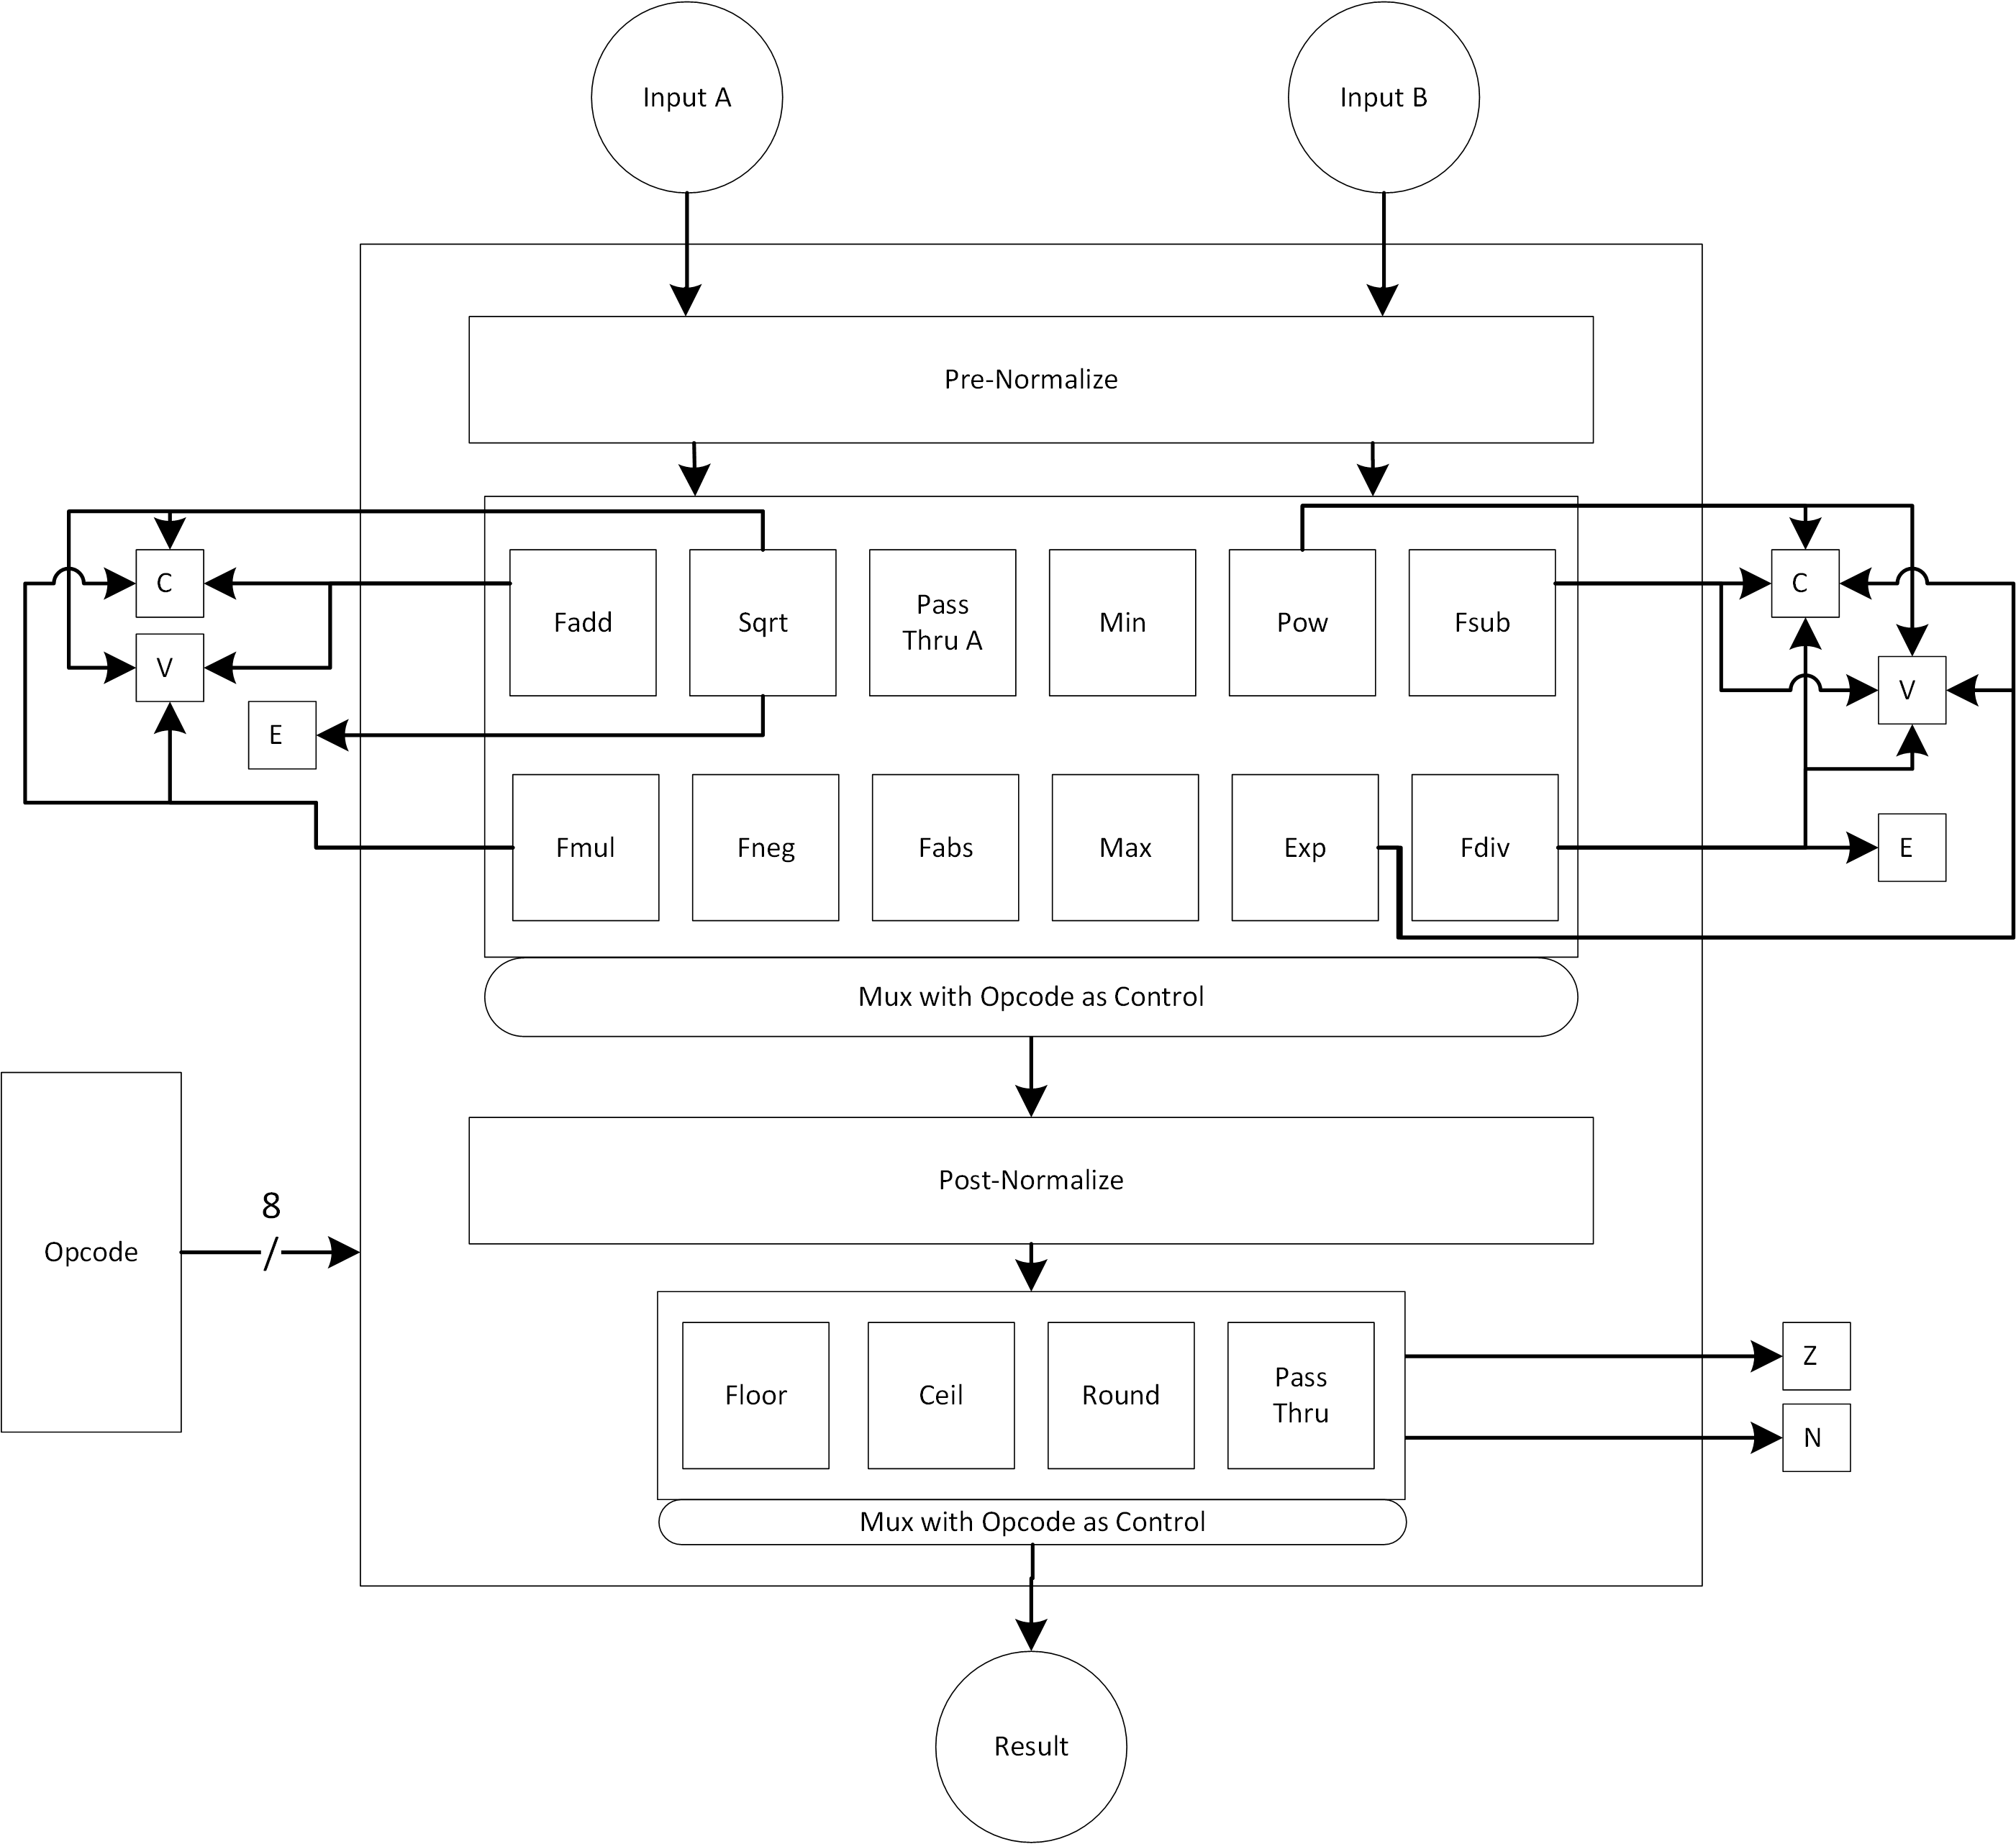
\includegraphics[width=1\linewidth]{ALU.png}
	\caption*{ALU Design}
	\end{center}
	\end{figure}

	\begin{landscape}
	\begin{figure}[H]
	\begin{center}
	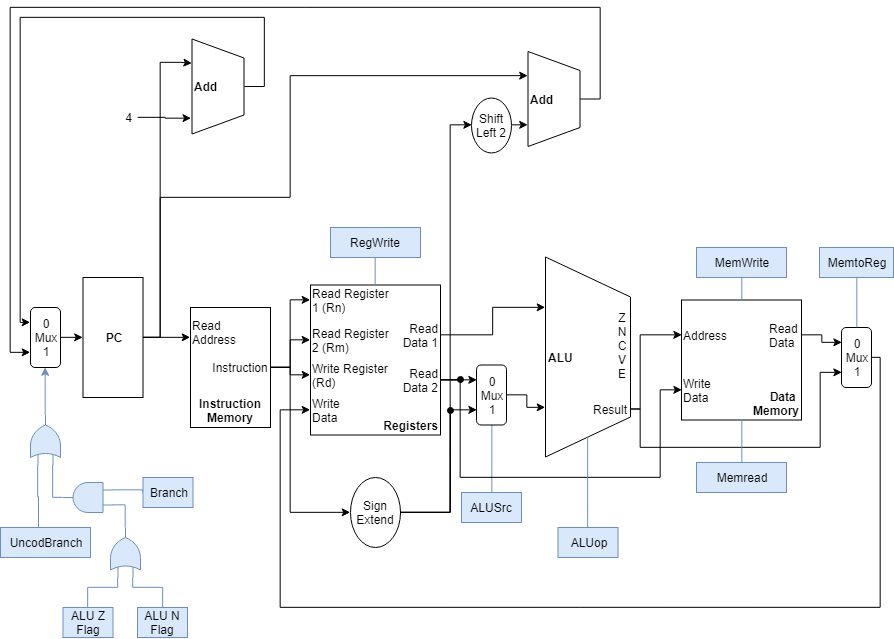
\includegraphics[width=1\linewidth]{SingleCycleArch.png}
	\caption*{Single Cycle Architecture}
	\end{center}
	\end{figure}
	\end{landscape}

	\begin{landscape}
	\begin{figure}[H]
	\begin{center}
	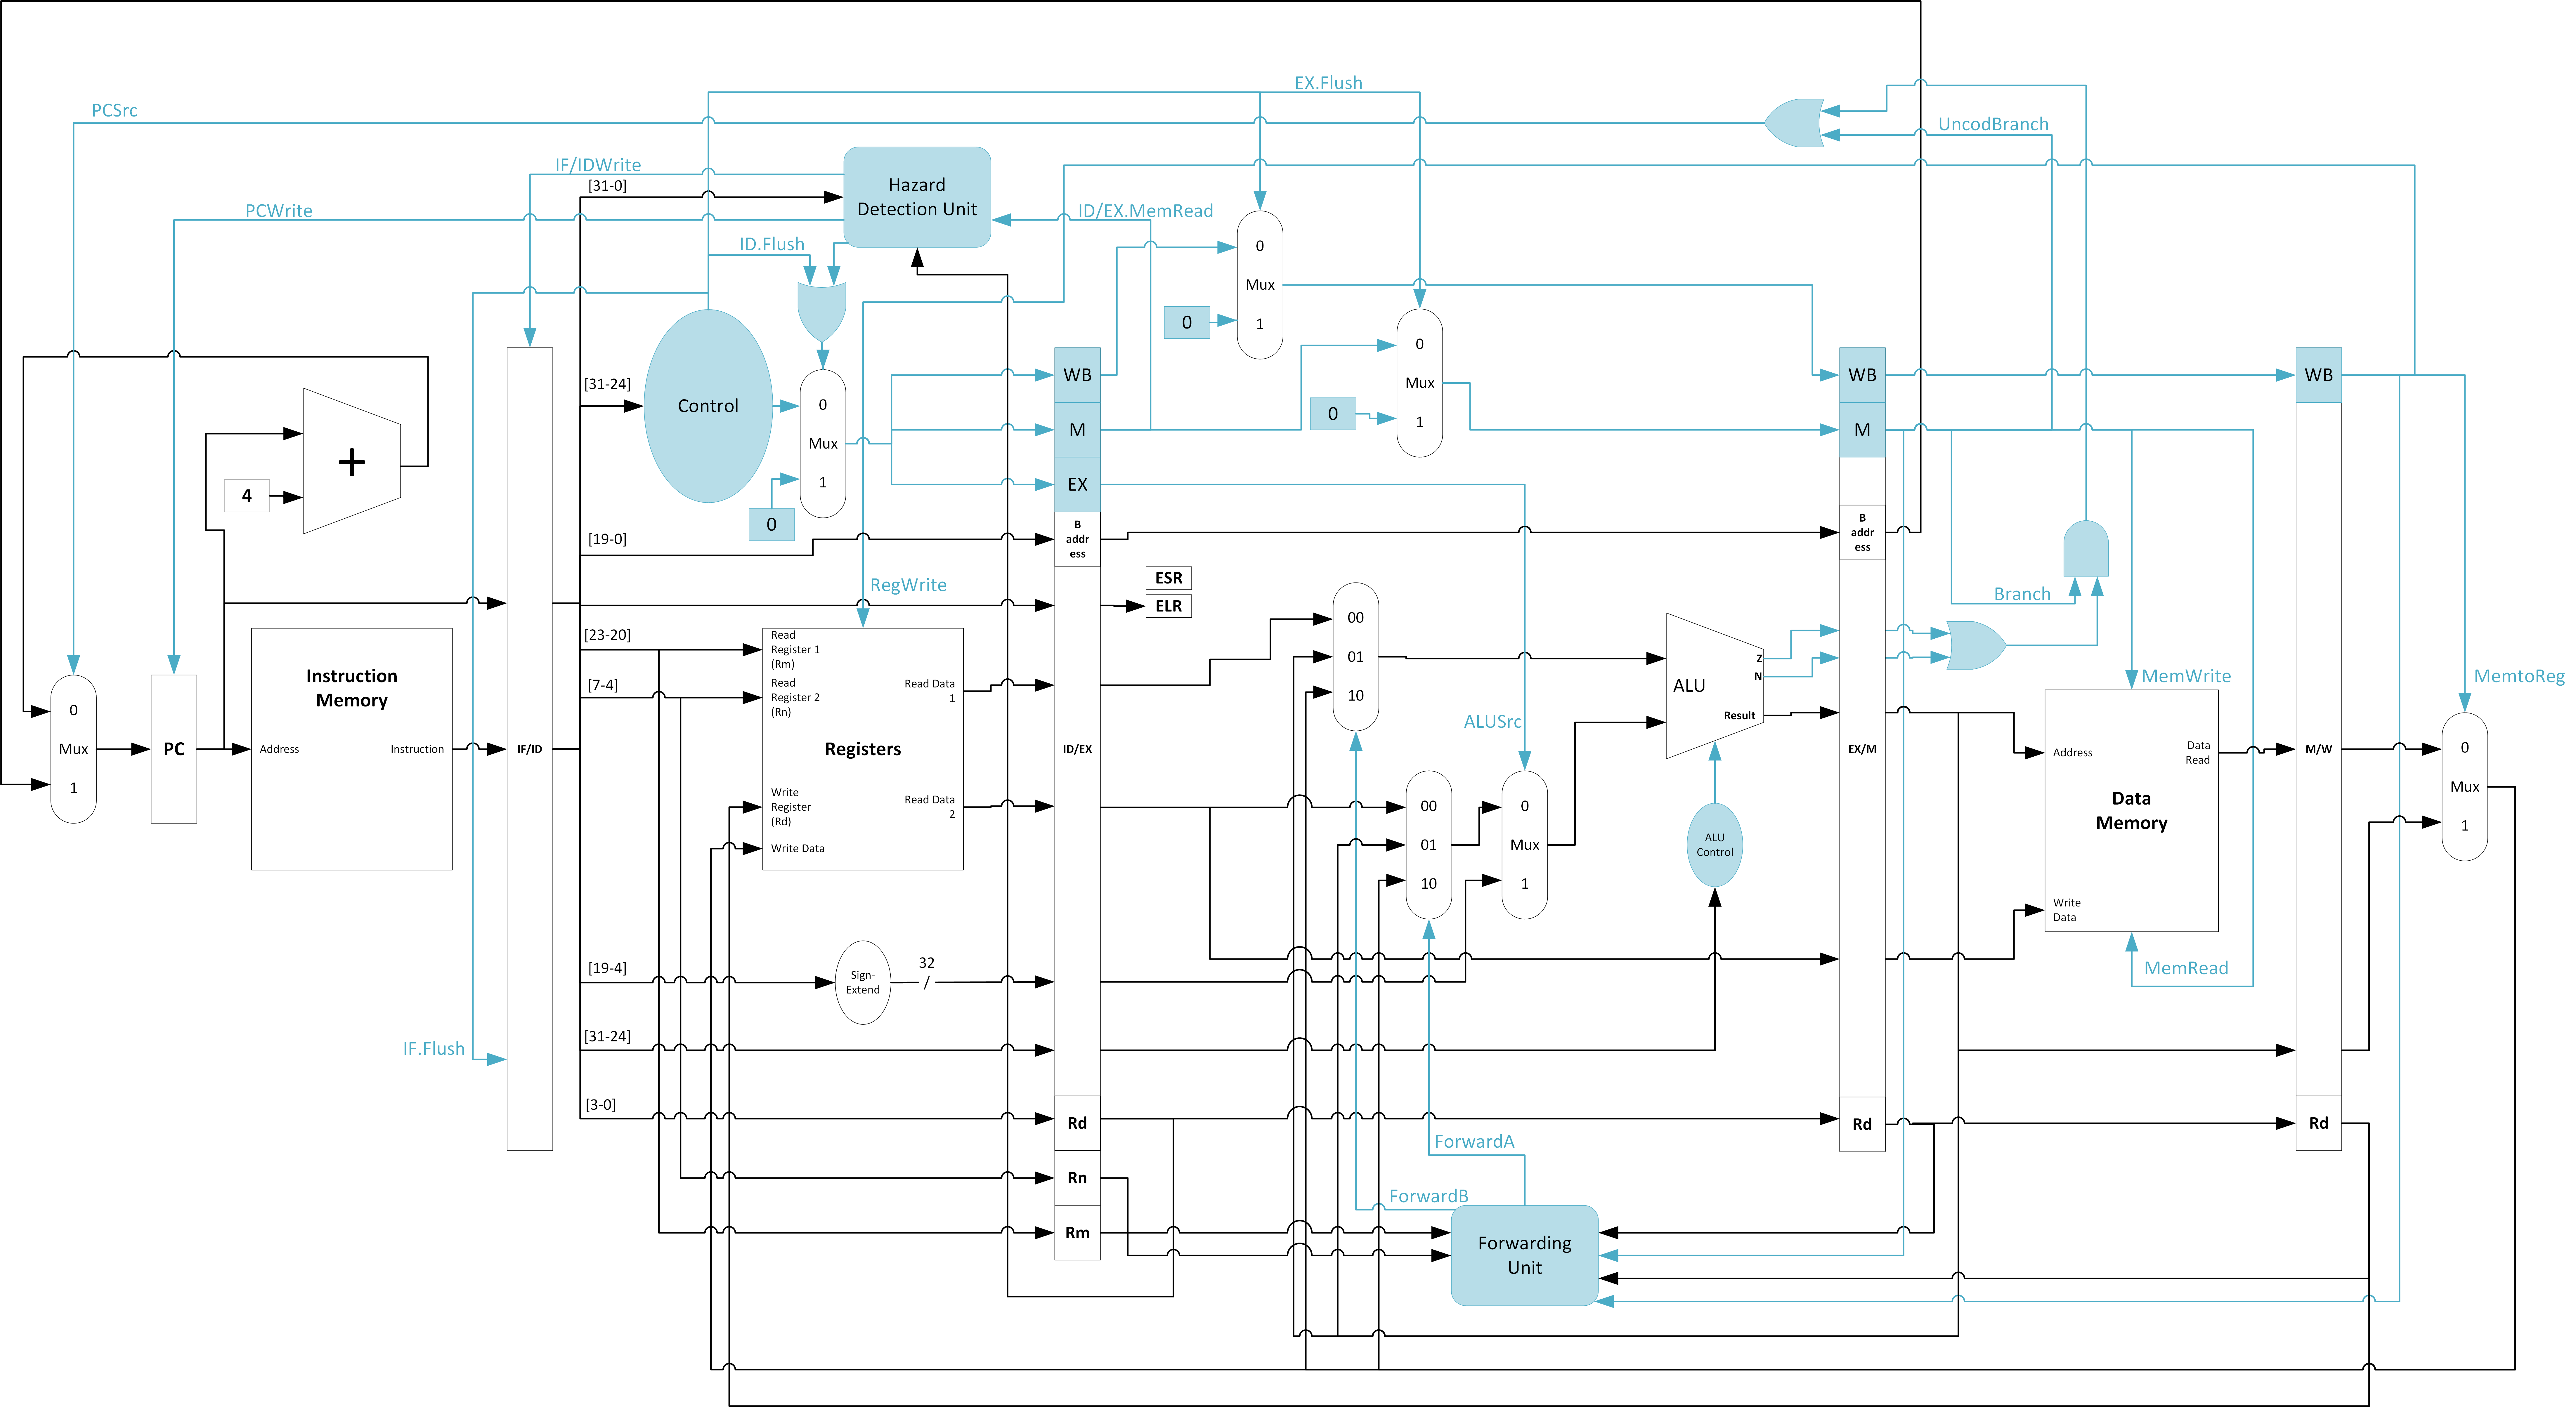
\includegraphics[width=1\linewidth]{PipelinedArch.png}
	\caption*{Pipelined Architecture}
	\end{center}
	\end{figure}
	\end{landscape}

\end{document}














